\hypertarget{main_8cpp}{
\section{main.cpp File Reference}
\label{main_8cpp}\index{main.cpp@{main.cpp}}
}
{\tt \#include $<$ptlib.h$>$}\par
{\tt \#include \char`\"{}cliview.h\char`\"{}}\par


Include dependency graph for main.cpp:\nopagebreak
\begin{figure}[H]
\begin{center}
\leavevmode
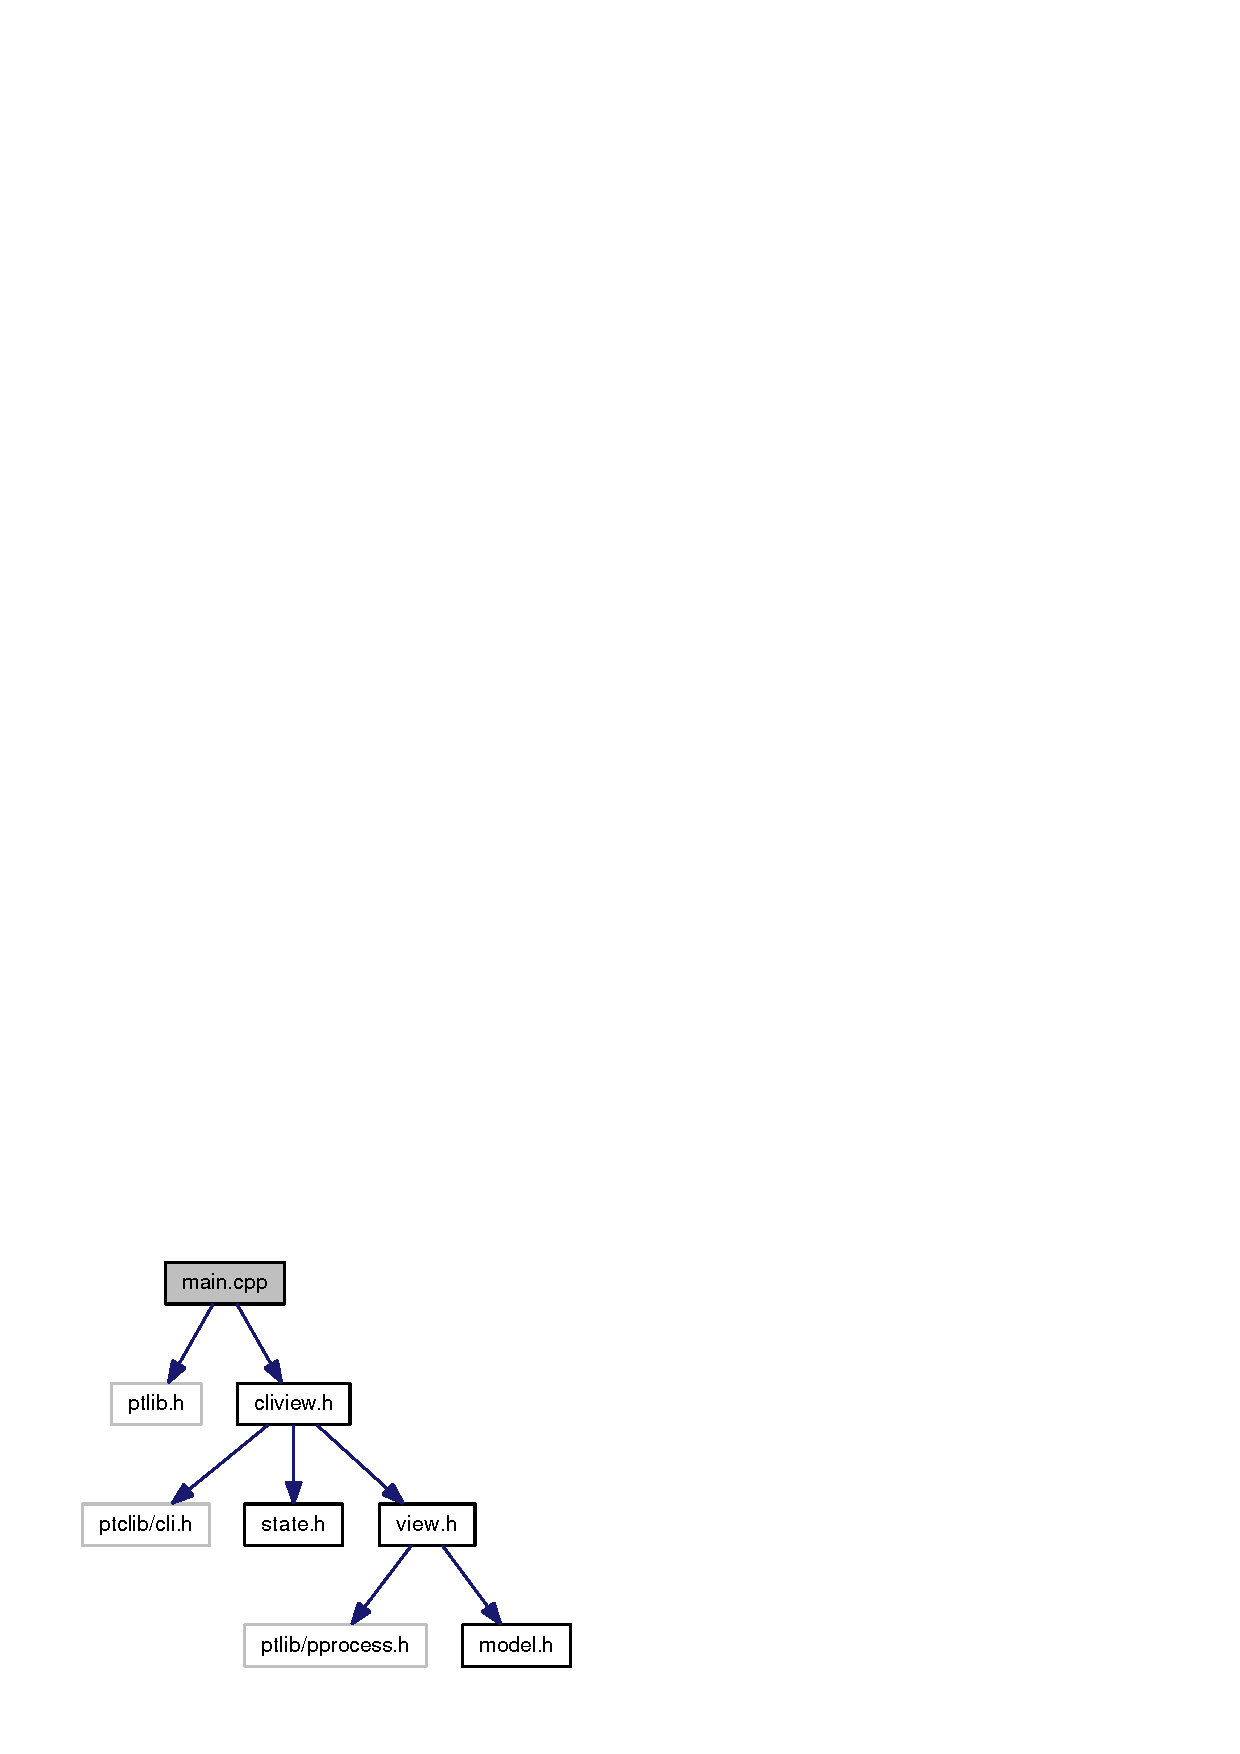
\includegraphics[width=139pt]{main_8cpp__incl}
\end{center}
\end{figure}
\subsection*{Functions}
\begin{CompactItemize}
\item 
\hyperlink{main_8cpp_7fdb2896b3ae3bf4fc9de267ce4999cd}{PCREATE\_\-PROCESS} (\hyperlink{classCLIView}{CLIView})
\begin{CompactList}\small\item\em The PCREATE\_\-PROCESS macro. \item\end{CompactList}\end{CompactItemize}


\subsection{Function Documentation}
\hypertarget{main_8cpp_7fdb2896b3ae3bf4fc9de267ce4999cd}{
\index{main.cpp@{main.cpp}!PCREATE\_\-PROCESS@{PCREATE\_\-PROCESS}}
\index{PCREATE\_\-PROCESS@{PCREATE\_\-PROCESS}!main.cpp@{main.cpp}}
\subsubsection[{PCREATE\_\-PROCESS}]{\setlength{\rightskip}{0pt plus 5cm}PCREATE\_\-PROCESS ({\bf CLIView})}}
\label{main_8cpp_7fdb2896b3ae3bf4fc9de267ce4999cd}


The PCREATE\_\-PROCESS macro. 

.. 1. Defines the main() function. 2. Creates an instance of \hyperlink{classTeleKarma}{TeleKarma}. 3. Calls instance-$>$PreInitialise() which is inherited from PProcess. 4. Calls instance-$>$InternalMain() which is inherited from PProcess. 5. instance-$>$InternalMain() calls instance-$>$Main() which must be defined in \hyperlink{classTeleKarma}{TeleKarma}. 